\documentclass{cranfieldChart}


\begin{document}

\maketitle{Group project - G2}
{Q. Diaferia\\
T. Levasseur\\
G. Perez Bada\\
P. Wang
}{Group project}{Group 2 - MeshSlicer}{cover.png}

\newpage
\tableofcontents
\listoffigures
\newpage

\begin{abstract}
The traditional way to write software application is serial, and instructions are executed on a single processor one after another.
As scientific simulation problem's size grows, this way becomes more and more time consuming and is no longer suitable. This is why we introduce the notion of parallel computing: the simultaneous use of multiple processors to solve a single and large size computational problem. One of the important approach to parallel computing is the distribution of memory and problem partitioning. Partitioning a problem can be challenging since the total work load should be divided in a way that processors share the same amount of work load and inter-processor communication time is minimized. In order to simplify the graph problem and so make the partitioning problem easier, we introduce another phase before computing the partition phase: coarsening phase, where a matching of edges is performed and vertices incident on these edges are collapsed together. We also introduce a final phase: refinement phase which reform the partitioned graph to it original form. Our work aims to address the challenge of partitioning graphs using open source libraries: METIS and ParMETIS. We conducted a website that enables users to connect to Astral resources remotely and partition their graphs online in a timely fashion. 
\end{abstract}

\section{Feasibility Analysis} 
Before specifying the requirements of this project, we first study its feasibility. That is, technical feasibility, economical feasibility and organisation feasibility. We first tested if the two applications that we would be using to partition graphs were working properly. Then, we made sure that our website prototype could connect users with their Astral ID and password remotely to Astral. Since the two partition applications are free, we are able to run this project without any financial restraint. We paid a visit to the Cranfield IT department to required whether it was possible for an external company to reach an agreement with Cranfield University to obtain extra Astral ID. The answer was no. So we fixed our target customers as those who already had Astral accounts. The only risk would lay on network connection. 

\section{High level description of our website}
This is a website application that enable user who hold a valid Cranfield Astral ID and password to upload graphs, select a partition method, choose an initial partition scheme, a refinement scheme, the number of parts in which to split the graph, set the maximum load imbalance, decide the weight of each partition and either they want to minimize edge cut or volume. 
Once the setting is finished, the partitioning will be done remotely on Astral and the results will be sent back to the web interface where our users will be able to collect the output files containing the partitioned graph as well as downloading them to their local PC. 

\section{Architecture of our system}
\begin{figure}[h]
\centering
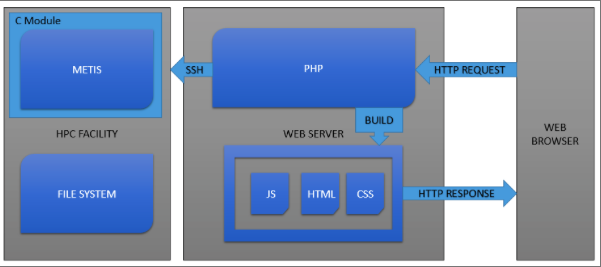
\includegraphics[width=0.8\textwidth]{ressources/architect}
\caption{System architecture}
\end{figure}
In general, our application is a web-based, three-tier, client-server system. On the client side, the web browser first send a http request to the web server in which the php script will interpret the request and remotely connect to the HPC faculty. Once the computation is done by $Metis$ which should be installed on the HPC faculty beforehand, the php script will build automatically a web page that contains JavaScript, HTML and CSS code. Finally, the web page will be display on the web browser. 
\section{Requirement Analysis} 
User requirement: \\
System functional requirements specification: \\
This a web application that allows users to partition graphs and mesh on-line in a timely fashion. 
\begin{itemize}
    \item The application shall allow user to log in with a valid Cranfield Astral user ID and password. 
    \item Once the user is logged in, the application shall allow him to upload graphs or meshes in form of $graph_name.graph$ and $mesh_name.mesh$ from his local PC. 
    \item The application shall be able to remotely use $MeTis$ as open sources for partitioning located on Astral system. 
    \item The application shall allow the user to select a partition method between k-way and recursive bisection.
     \item The application shall let the user set either if he wants to minimize the edge cut or communication of the graph.
    \item The application shall allow the user to choose one initial partition scheme between:
        \begin{itemize}
             \item Greedy bisection
            \item Random bisection and refinement 
        \end{itemize}
    \item The application shall allow the user to choose on coarsening method between: 
        \begin{itemize}
            \item Random matching 
            \item Heavy edge cutting 
        \end{itemize}
    \item The application shall allow user to set if the partition is contiguous or not. 
    \item The application shall allow user to set the maximum load imbalance via x with $L= (1+x)/100$
    \item The application shall let the user set the number of parts in which to split the graph. 
    \item If the user choose to partition a mesh, the user shall be able to mesh type between: 
    \begin{itemize}
        \item Dual Graph
        \item Nodal Graph 
    \end{itemize}
    \item Once the user finish setting the partition preferences and click on the launch partition, a video window will pop up and he or she shall be able to view the whole partitioning process as the origin graph will be painted on different colors which represents different partition group. 
    \item The application shall allow users to download the output file to his local PC. Original output file of the $Metis$ application contains only one index number on each line which represents a node of the graph and the index number means the processor to which it has been assigned. 
    \item User shall be able to delete any file from his repository. 
    \item User shall be able to log out at any time. 
    \end{itemize}
    System non functional requirements specification: 
    \begin{itemize}
        \item Users' log in security should be verified. User's ID and password shouldn't be given out under any circumstances. 
        \item The application respond time shall be in order of second. 
        \item The application shall be easy to use without tutorial needed, but description of different partition methods and refinement schemes shall be included on the website. 
        \item The application shall be working 24h/24h per day and 7 days per week and downtime shall not exceed 30 secs. 
     \end{itemize}
\section{Usage of tools}
We decided to use $Metis$ and $ParMetis$ as open sources to compute data partition. They are well known for producing high quality partitions in a timely fashion and being actively supported. 
\section{Use case diagram}
\begin{figure}[h]
\centering
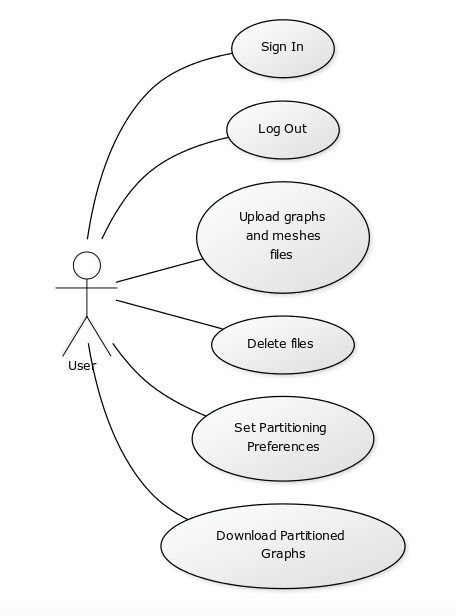
\includegraphics[width=0.8\textwidth]{ressources/use-case}
\caption{Use case diagram}
\end{figure}
Use case diagram specification: \\
We define only user as actor in our system as we use remotely Astral resource to control access, manage users' information and users' input and output files. In general, our web application serves as a platform to enable users to connect remotely to Astral and use its resources. ($Metis$ in our case) \\
Definition of actions: 
\begin{itemize}
    \item Sign in 
    \item Log out
    \item Upload graphs and meshes
    \item Set Partitioning Preferences 
    \item Download Partitioned Graphs 
\end{itemize}
As described earlier, our users shall be able to set the partition preferences. The setting requirements are predefined on $Metis$ as input parameters. Our job is to provide a link between the web interface and $Metis$ so that the setting preferences will be used as configuration input to launch the partitioning on $Metis$. Setting parameters are as followed:\\ 
\begin{itemize}
    \item Graph/Mesh 
    \begin{itemize}
        \item Graph:0
        \item Mesh: 1
    \end{itemize}
    \item Partition method
    \begin{itemize}
        \item Bisection:0
        \item K-way: 1
    \end{itemize}
    \item Partition objective
    \begin{itemize}
        \item Edge cut: 0
        \item Communication volume: 1
    \end{itemize}
    \item Coarsening scheme
    \begin{itemize}
        \item Random: 0
        \item Heavy-edge : 1
    \end{itemize}
    \item  Initial partition scheme
    \begin{itemize}
        \item Greedy: 0
        \item Random bisection + refinement: 1
        \item Edge cut derived: 2
        \item Node-based greedy: 3
    \end{itemize}
    \item Contiguous partition
    \begin{itemize}
        \item No: 0
        \item Yes: 1
    \end{itemize}
    \item Imbalance value $x$
    \begin{itemize}
        \item Default: 0
        \item Integer: $x$
    \end{itemize}
    \item Number of parts 
    \item Mesh based
    \begin{itemize}
        \item Dual graph: 0
        \item Nodes: 1
    \end{itemize}
    
\end{itemize}
\section{How we manage the project and tasks partition}
After our first meeting, we first analysed the total work load of the project and established a to-do list. We exchanged each group member's strengths and divided tasks accordingly. We used $Trello$ and $GitHub$ as real-time monitoring tools for group file management and we defined our to-do tasks as followed: \\
\begin{itemize}
    \item Development of web interface 
    \item Development of an algorithm which establishes the connection between Astral and our web interface. Once our user set the graph partition's preferences, those input would pass automatically as parameters to $Metis$. On the other hand, when the partitioning is finished, the output file should be sent back to our web interface. 
     \item Development of an algorithm that takes the original $.graph$ file and the output file generated by $Metis$ as input, and compute a dynamic graphic presentation of the graph partition. In the end, all the nodes in the graph will be painted with different color which indicates the partition. 
     \item In order to display the partitioning process graphically for large size graph, an algorithm has to be built. The basic idea of this program is to regroup nodes that are connected to each other randomly.   
\end{itemize}
\subsection{Partition of tasks} 
Quentin, who has a background of developing web application using php and JavaScript is in charge of developing the web interface that enable users to: 
\begin{itemize}
    \item Sign in 
    \item Upload files from local PC 
    \item Download files from web application 
\end{itemize}
Thibaud, who is also familiar with JavaScript is in charge with: 
\begin{itemize}
    \item Developing an algorithm that reduce the size of graph and using $SigmaJs$ library.
    \item Developing an algorithm that combine the original input graph file and the output file generated by $Metis$ in order to generate a dynamic graphic presentation of the graph partition. 
\end{itemize}
Gonzalo, who feels comfortable of using Astral remotely, volunteer to develop a program which connects Astral and our website interface. \\
And Pei is responsible for, 
\begin{itemize}
    \item Analysing requirements and design patterns. 
    \item Designing the advertisement flyer.
    \item Writing  the project report.
    \item Organise the presentation 
\end{itemize}

\section{Results}
\begin{figure}[h]
\centering
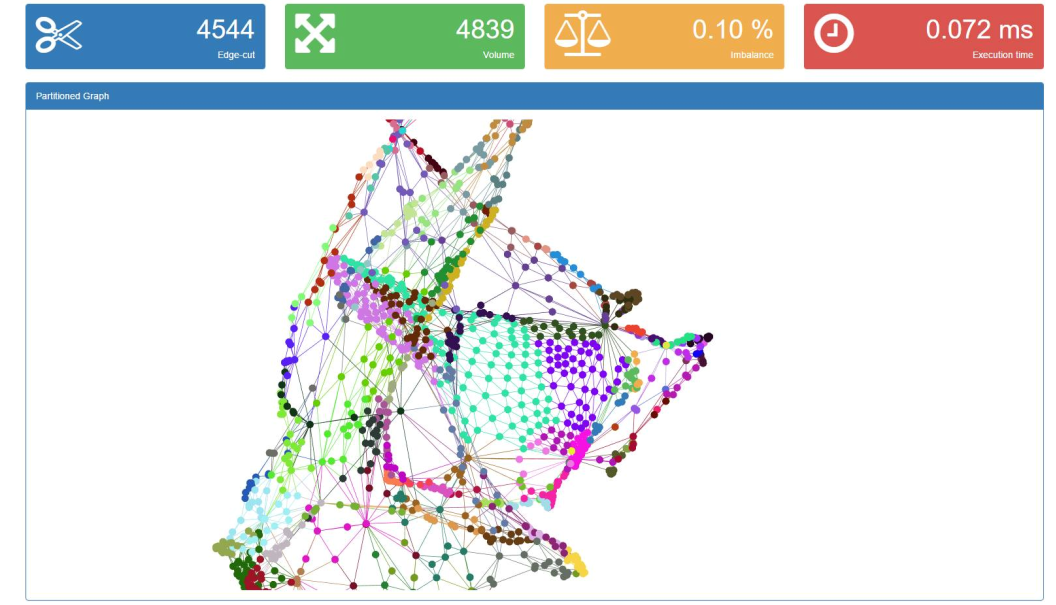
\includegraphics[width=0.8\textwidth]{ressources/graph}
\caption{result example}
\end{figure}
One can see from above, nodes on the graph are painted into different color which indicates the partition. The edge-cut value, volume value, imbalance value is calculated and displayed as well as the execution time which is in order of second. 


\end{document}